% !TEX program = xelatex
\documentclass[aspectratio=169]{beamer}
\usepackage{amsmath}
\usepackage{amssymb}
\usepackage{graphicx}
\usepackage{tcolorbox}
\usepackage{booktabs}
\usepackage{colortbl}
\usepackage{xcolor}
\usepackage{tikz}
\usetikzlibrary{angles,quotes}
\usepackage[utf8]{inputenc}

% Custom colors
\definecolor{primary}{RGB}{41, 128, 185}
\definecolor{secondary}{RGB}{52, 152, 219}
\definecolor{accent}{RGB}{231, 76, 60}
\definecolor{lightgray}{RGB}{236, 240, 241}

% Theme customization
\usetheme{Madrid}
\usecolortheme{whale}
\setbeamercolor{structure}{fg=primary}
\setbeamercolor{background canvas}{bg=white}
\setbeamercolor{normal text}{fg=black}

% Title page info
\title{Pre-Calculus 11}
\subtitle{Solving for Angles in All Four Quadrants}
\author{Created by Yi-Chen Lin}
\date{\today}

\begin{document}

% Title Page
\begin{frame}
    \titlepage
\end{frame}

% I) REVIEW: SOH-CAH-TOA
\begin{frame}{Review: SOH-CAH-TOA}
    \begin{tcolorbox}[colback=lightgray,colframe=primary,title=Key Trig Ratios]
        \footnotesize
        \begin{columns}
            \column{0.6\textwidth}
            \begin{align*}
                \sin \theta &= \frac{\text{Opposite}}{\text{Hypotenuse}} \\
                \cos \theta &= \frac{\text{Adjacent}}{\text{Hypotenuse}} \\
                \tan \theta &= \frac{\text{Opposite}}{\text{Adjacent}}
            \end{align*}
            \begin{itemize}
                \item Pythagorean Theorem: $a^2 + b^2 = c^2$
                \item Circle Equation: $x^2 + y^2 = r^2$
            \end{itemize}
            \column{0.4\textwidth}
            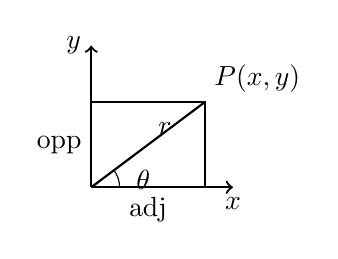
\begin{tikzpicture}[scale=0.9]
                \draw[thick,->] (0,0) -- (2,0) node[below]{$x$};
                \draw[thick,->] (0,0) -- (0,2) node[left]{$y$};
                \draw[thick] (0,0) -- (1.6,1.2) node[midway, above right]{$r$};
                \draw[thick] (1.6,0) -- (1.6,1.2) -- (0,1.2);
                \node[below] at (0.8,0) {adj};
                \node[left] at (0,0.6) {opp};
                \node[above right] at (1.6,1.2) {$P(x,y)$};
                \draw (0.4,0) arc (0:37:0.4);
                \node[right] at (0.5,0.1) {$\theta$};
            \end{tikzpicture}
        \end{columns}
    \end{tcolorbox}
\end{frame}

% II) Trig Ratio for Any Angle
\begin{frame}{Trig Ratio for Any Angle}
    \begin{tcolorbox}[colback=lightgray,colframe=accent,title=Coordinates on the Circle]
        \footnotesize
        \begin{columns}
            \column{0.6\textwidth}
            \begin{itemize}
                \item For angle $\theta$ in standard position, any point $P(x, y)$ on the circle of radius $r$:
                \item $x = r \cos \theta$, $y = r \sin \theta$
                \item On the unit circle ($r=1$): $P(\cos\theta, \sin\theta)$
            \end{itemize}
            \column{0.4\textwidth}
            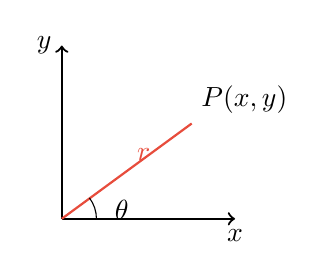
\begin{tikzpicture}[scale=1.1]
                \draw[thick,->] (0,0) -- (2,0) node[below]{$x$};
                \draw[thick,->] (0,0) -- (0,2) node[left]{$y$};
                \draw[thick,accent] (0,0) -- (1.5,1.1) node[midway, above right]{$r$};
                \node[above right] at (1.5,1.1) {$P(x,y)$};
                \draw (0.4,0) arc (0:37:0.4);
                \node[right] at (0.5,0.1) {$\theta$};
            \end{tikzpicture}
        \end{columns}
    \end{tcolorbox}
\end{frame}

% Example: Find coordinates for given angles
\begin{frame}{Example: Coordinates for Given Angles}
    \begin{tcolorbox}[colback=lightgray,colframe=primary,title=Question]
        \footnotesize
        Find the coordinates of point $P(x,y)$ for the following angles in standard position:
        \begin{itemize}
            \item $\theta = 215^\circ$
            \item $\theta = 150^\circ$
        \end{itemize}
    \end{tcolorbox}
\end{frame}

\begin{frame}{Example: Coordinates for Given Angles}
    \begin{tcolorbox}[colback=lightgray,colframe=primary,title=Solution]
        \footnotesize
        \begin{itemize}
            \item $\theta = 215^\circ$: $x = \cos 215^\circ \approx -0.819$, $y = \sin 215^\circ \approx -0.573$
            \item $\theta = 150^\circ$: $x = \cos 150^\circ \approx -0.866$, $y = \sin 150^\circ \approx 0.5$
        \end{itemize}
    \end{tcolorbox}
\end{frame}

% IV) Sine/Cosine/Tangent in Different Quadrants (CAST)
\begin{frame}{Sine, Cosine, Tangent in Different Quadrants}
    \begin{tcolorbox}[colback=lightgray,colframe=accent,title=CAST Rule]
        \footnotesize
        \begin{columns}
            \column{0.6\textwidth}
            \begin{itemize}
                \item Sine, cosine, and tangent can be positive or negative depending on the quadrant.
                \item Use the CAST rule to remember which is positive:
            \end{itemize}
            \begin{itemize}
                \item Quadrant I: All positive
                \item Quadrant II: Sine only
                \item Quadrant III: Tangent only
                \item Quadrant IV: Cosine only
            \end{itemize}
            \column{0.4\textwidth}
            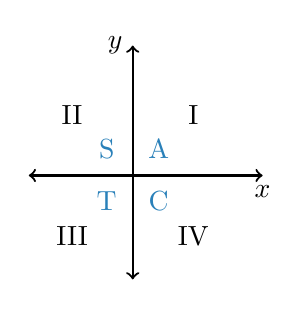
\begin{tikzpicture}[scale=1.1]
                \draw[thick,->] (0,0) -- (1.5,0) node[below]{$x$};
                \draw[thick,->] (0,0) -- (0,1.5) node[left]{$y$};
                \draw[thick,->] (0,0) -- (-1.2,0);
                \draw[thick,->] (0,0) -- (0,-1.2);
                \node at (0.7,0.7) {I};
                \node at (-0.7,0.7) {II};
                \node at (-0.7,-0.7) {III};
                \node at (0.7,-0.7) {IV};
                \node[primary] at (0.3,0.3) {A};
                \node[primary] at (-0.3,0.3) {S};
                \node[primary] at (-0.3,-0.3) {T};
                \node[primary] at (0.3,-0.3) {C};
            \end{tikzpicture}
        \end{columns}
    \end{tcolorbox}
\end{frame}

% Example: Which Quadrant?
\begin{frame}{Example: Which Quadrant?}
    \begin{tcolorbox}[colback=lightgray,colframe=primary,title=Question]
        \footnotesize
        Determine which quadrants the angle $\theta$ can be in for the following trig functions:
        \begin{itemize}
            \item $\sin\theta = -2/3$
            \item $\cos\theta = 2/5$
            \item $\tan\theta = -3/7$
        \end{itemize}
    \end{tcolorbox}
\end{frame}

\begin{frame}{Example: Which Quadrant?}
    \begin{tcolorbox}[colback=lightgray,colframe=primary,title=Solution]
        \footnotesize
        \begin{itemize}
            \item $\sin\theta = -2/3$ (negative): $\theta$ in Q3 & Q4
            \item $\cos\theta = 2/5$ (positive): $\theta$ in Q1 & Q4
            \item $\tan\theta = -3/7$ (negative): $\theta$ in Q2 & Q4
        \end{itemize}
    \end{tcolorbox}
\end{frame}

% Steps for Solving for Angles
\begin{frame}{Steps for Solving for Angles}
    \begin{tcolorbox}[colback=lightgray,colframe=accent,title=Step-by-Step]
        \footnotesize
        \begin{enumerate}
            \item Identify the trig function (sine, cosine, tangent)
            \item Check if the ratio is positive or negative
            \item Use CAST to determine possible quadrants
            \item Use inverse trig to find the reference angle
            \item Find the second angle in the other quadrant
            \item State both solutions
        \end{enumerate}
    \end{tcolorbox}
\end{frame}

% Example: Solve for the angle (sinθ = 2/5)
\begin{frame}{Example: Solve for the Angle}
    \begin{tcolorbox}[colback=lightgray,colframe=primary,title=Question]
        \footnotesize
        Solve for $\theta$ given $\sin\theta = 2/5$.
    \end{tcolorbox}
\end{frame}

\begin{frame}{Example: Solve for the Angle}
    \begin{tcolorbox}[colback=lightgray,colframe=primary,title=Solution]
        \footnotesize
        $\sin\theta = 2/5$ (positive)\\
        $\theta$ in Q1 and Q2\\
        $\theta_1 = \sin^{-1}(2/5) \approx 23.58^\circ$\\
        $\theta_2 = 180^\circ - 23.58^\circ = 156.42^\circ$
        
        \begin{center}
        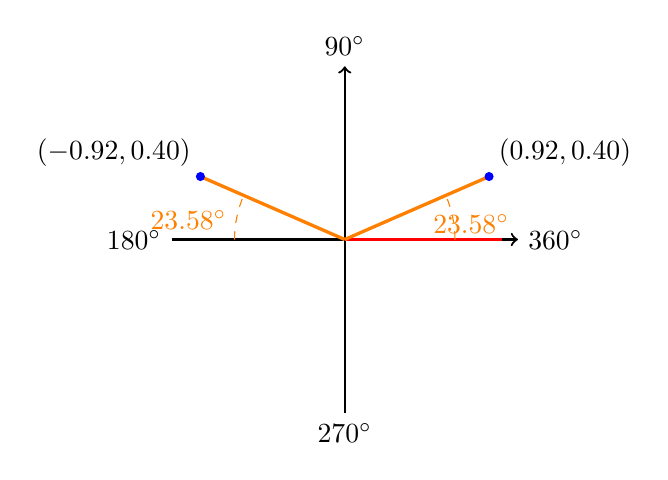
\begin{tikzpicture}[scale=2]
          % Axes
          \draw[thick,->] (-1.1,0) -- (1.1,0) node[right] {$360^\circ$};
          \draw[thick,->] (0,-1.1) -- (0,1.1) node[above] {$90^\circ$};
          \draw[thick] (-1,0) -- (-1.1,0) node[left] {$180^\circ$};
          \draw[thick] (0,-1) -- (0,-1.1) node[below] {$270^\circ$};
          % Initial arm
          \draw[very thick,red] (0,0) -- (1,0);
          % Terminal arm Q1
          \draw[very thick,orange] (0,0) -- ({cos(23.58)},{sin(23.58)});
          % Terminal arm Q2
          \draw[very thick,orange] (0,0) -- ({cos(156.42)},{sin(156.42)});
          % Reference angle arc Q1
          \draw[dashed,orange] (0.7,0) arc (0:23.58:0.7);
          % Reference angle arc Q2
          \draw[dashed,orange] ({0.7*cos(180)},{0.7*sin(180)}) arc (180:156.42:0.7);
          % Points
          \filldraw[blue] ({cos(23.58)},{sin(23.58)}) circle (0.025);
          \filldraw[blue] ({cos(156.42)},{sin(156.42)}) circle (0.025);
          % Labels
          \node[above right] at ({cos(23.58)},{sin(23.58)}) {$(0.92,0.40)$};
          \node[above left] at ({cos(156.42)},{sin(156.42)}) {$(-0.92,0.40)$};
          \node[orange,right] at (0.5,0.1) {$23.58^\circ$};
          \node[orange,left] at ({0.7*cos(170)},{0.7*sin(170)}) {$23.58^\circ$};
        \end{tikzpicture}
        \end{center}
    \end{tcolorbox}
\end{frame}

% Example: Solve for the angle (cosθ = -3/7)
\begin{frame}{Example: Solve for the Angle (Cos Negative)}
    \begin{tcolorbox}[colback=lightgray,colframe=primary,title=Question]
        \footnotesize
        Solve for $\theta$ given $\cos\theta = -3/7$.
    \end{tcolorbox}
\end{frame}

\begin{frame}{Example: Solve for the Angle (Cos Negative)}
    \begin{tcolorbox}[colback=lightgray,colframe=primary,title=Solution]
        \footnotesize
        $\cos\theta = -3/7$ (negative)\\
        $\theta$ in Q2 and Q3\\
        $\theta_1 = \cos^{-1}(-3/7) \approx 115.54^\circ$\\
        $\theta_2 = 360^\circ - 115.54^\circ = 244.46^\circ$
        
        \begin{center}
        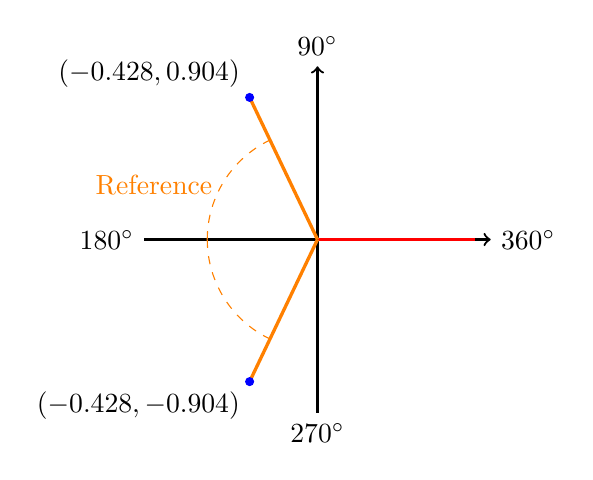
\begin{tikzpicture}[scale=2]
          % Axes
          \draw[thick,->] (-1.1,0) -- (1.1,0) node[right] {$360^\circ$};
          \draw[thick,->] (0,-1.1) -- (0,1.1) node[above] {$90^\circ$};
          \draw[thick] (-1,0) -- (-1.1,0) node[left] {$180^\circ$};
          \draw[thick] (0,-1) -- (0,-1.1) node[below] {$270^\circ$};
          % Initial arm
          \draw[very thick,red] (0,0) -- (1,0);
          % Terminal arm Q2
          \draw[very thick,orange] (0,0) -- ({cos(115.54)},{sin(115.54)});
          % Terminal arm Q3
          \draw[very thick,orange] (0,0) -- ({cos(244.46)},{sin(244.46)});
          % Reference angle arc Q2
          \draw[dashed,orange] ({0.7*cos(180)},{0.7*sin(180)}) arc (180:115.54:0.7);
          % Reference angle arc Q3
          \draw[dashed,orange] ({0.7*cos(180)},{0.7*sin(180)}) arc (180:244.46:0.7);
          % Points
          \filldraw[blue] ({cos(115.54)},{sin(115.54)}) circle (0.025);
          \filldraw[blue] ({cos(244.46)},{sin(244.46)}) circle (0.025);
          % Labels
          \node[above left] at ({cos(115.54)},{sin(115.54)}) {$(-0.428,0.904)$};
          \node[below left] at ({cos(244.46)},{sin(244.46)}) {$(-0.428,-0.904)$};
          \node[orange,left] at ({0.7*cos(150)},{0.7*sin(150)}) {Reference};
        \end{tikzpicture}
        \end{center}
    \end{tcolorbox}
\end{frame}

% Example: tanθ = 4/9
\begin{frame}{Example: $\tan\theta = 4/9$}
    \begin{tcolorbox}[colback=lightgray,colframe=primary,title=Question]
        \footnotesize
        Given $\tan\theta = 4/9$, find all possible coordinates for point $P(x,y)$ in the unit circle.
    \end{tcolorbox}
\end{frame}

\begin{frame}{Example: $\tan\theta = 4/9$}
    \begin{tcolorbox}[colback=lightgray,colframe=primary,title=Solution]
        \footnotesize
        $\tan\theta = 4/9$ (positive)\\
        $\theta$ in Q1 and Q3\\
        $x = 0.917$, $y = 0.401$ (Q1), $x = -0.917$, $y = -0.401$ (Q3)\\
        \textbf{Reference angle:} $\theta_1 = \tan^{-1}(4/9) \approx 23.96^\circ$\\
        $\theta_2 = 180^\circ + 23.96^\circ = 203.96^\circ$
        
        \begin{center}
        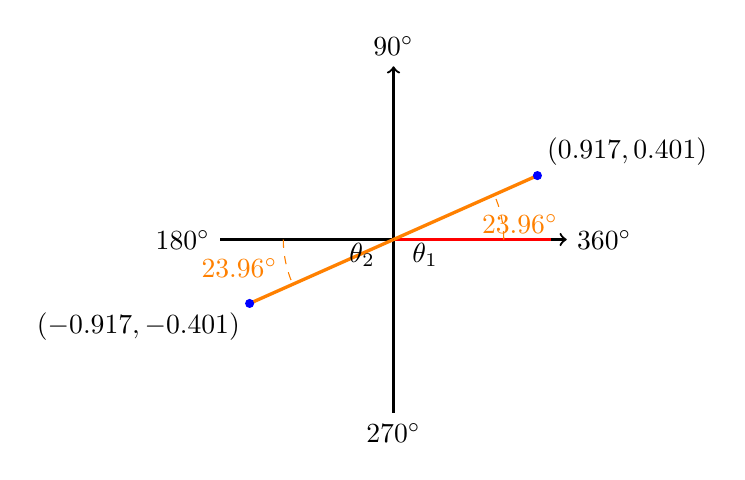
\begin{tikzpicture}[scale=2]
          % Axes
          \draw[thick,->] (-1.1,0) -- (1.1,0) node[right] {$360^\circ$};
          \draw[thick,->] (0,-1.1) -- (0,1.1) node[above] {$90^\circ$};
          \draw[thick] (-1,0) -- (-1.1,0) node[left] {$180^\circ$};
          \draw[thick] (0,-1) -- (0,-1.1) node[below] {$270^\circ$};
          % Initial arm
          \draw[very thick,red] (0,0) -- (1,0);
          % Terminal arm Q1
          \draw[very thick,orange] (0,0) -- ({cos(23.96)},{sin(23.96)});
          % Terminal arm Q3
          \draw[very thick,orange] (0,0) -- ({cos(203.96)},{sin(203.96)});
          % Reference angle arc Q1
          \draw[dashed,orange] (0.7,0) arc (0:23.96:0.7);
          % Reference angle arc Q3
          \draw[dashed,orange] ({0.7*cos(180)},{0.7*sin(180)}) arc (180:203.96:0.7);
          % Points
          \filldraw[blue] ({cos(23.96)},{sin(23.96)}) circle (0.025);
          \filldraw[blue] ({cos(203.96)},{sin(203.96)}) circle (0.025);
          % Labels
          \node[above right] at ({cos(23.96)},{sin(23.96)}) {$(0.917,0.401)$};
          \node[below left] at ({cos(203.96)},{sin(203.96)}) {$(-0.917,-0.401)$};
          \node[orange,right] at (0.5,0.1) {$23.96^\circ$};
          \node[orange,left] at ({0.7*cos(195)},{0.7*sin(195)}) {$23.96^\circ$};
          \node at (0.2,-0.1) {$\theta_1$};
          \node at (-0.2,-0.1) {$\theta_2$};
        \end{tikzpicture}
        \end{center}
    \end{tcolorbox}
\end{frame}

% Practice: Find the Angles
\begin{frame}{Practice: Find the Angles}
    \begin{tcolorbox}[colback=lightgray,colframe=accent,title=Practice]
        \footnotesize
        Given $0^\circ \leq \theta \leq 360^\circ$, find the angles:
        \begin{itemize}
            \item $\tan\theta = -2/5$
            \item $\sin\theta = -5/3$
            \item $\cos\theta = -5/3$
        \end{itemize}
    \end{tcolorbox}
\end{frame}

% Q: One or No Solution?
\begin{frame}{Q: One or No Solution?}
    \begin{tcolorbox}[colback=lightgray,colframe=primary,title=Concept Check]
        \footnotesize
        Which of the following have one solution? Which have none?
        \begin{itemize}
            \item $\sin\theta = 0.856$
            \item $\sin\theta = 1$
            \item $\cos\theta = 1$
            \item $\cos\theta = 2.345$
            \item $\tan\theta = -9.856$
            \item $\tan\theta = 0$
            \item $\sin\theta = -1$
        \end{itemize}
    \end{tcolorbox}
\end{frame}

% Solving Trig Equations with Algebra
\begin{frame}{Solving Trig Equations with Algebra}
    \begin{tcolorbox}[colback=lightgray,colframe=accent,title=Steps]
        \footnotesize
        \begin{enumerate}
            \item Isolate the trig function
            \item Determine possible quadrants using CAST
            \item Find the reference angle
            \item State all solutions
        \end{enumerate}
    \end{tcolorbox}
\end{frame}

% Example: Algebraic Trig Equation
\begin{frame}{Example: Algebraic Trig Equation}
    \begin{tcolorbox}[colback=lightgray,colframe=primary,title=Question]
        \footnotesize
        Solve for $\theta$ given $8\sin\theta + 7 = 12$.
    \end{tcolorbox}
\end{frame}

\begin{frame}{Example: Algebraic Trig Equation}
    \begin{tcolorbox}[colback=lightgray,colframe=primary,title=Solution]
        \footnotesize
        $8\sin\theta + 7 = 12$\par
        $8\sin\theta = 5$\par
        $\sin\theta = 5/8$\par
        $\theta$ in Q1 and Q2\par
        $\theta_1 = \sin^{-1}(5/8) \approx 38.68^\circ$\par
        $\theta_2 = 180^\circ - 38.68^\circ = 141.32^\circ$
    \end{tcolorbox}
\end{frame}

% Practice: Solve for Theta
\begin{frame}{Practice: Solve for $\theta$}
    \begin{tcolorbox}[colback=lightgray,colframe=accent,title=Practice]
        \footnotesize
        Given $0^\circ \leq \theta \leq 360^\circ$, solve:
        \begin{itemize}
            \item $5\cos\theta + 13 = 11$
            \item $3\cos\theta = 8\sin\theta$
            \item $4\tan^2\theta + 7 = 10$
            \item $9\sin^2\theta - 4 = 0$
        \end{itemize}
    \end{tcolorbox}
\end{frame}

% SCT of 0, 90, 180, 270, 360
\begin{frame}{Sine, Cosine, Tangent of 0°, 90°, 180°, 270°, 360°}
    \begin{tcolorbox}[colback=lightgray,colframe=primary,title=Special Angles]
        \footnotesize
        \begin{itemize}
            \item $\sin\theta$ is the $y$-coordinate, $\cos\theta$ is the $x$-coordinate
            \item $\cos 0^\circ = 1$, $\sin 0^\circ = 0$
            \item $\cos 90^\circ = 0$, $\sin 90^\circ = 1$
            \item $\cos 180^\circ = -1$, $\sin 180^\circ = 0$
            \item $\cos 270^\circ = 0$, $\sin 270^\circ = -1$
            \item $\cos 360^\circ = 1$, $\sin 360^\circ = 0$
        \end{itemize}
    \end{tcolorbox}
\end{frame}

% Q: What is tanθ at these angles?
\begin{frame}{What is $\tan\theta$ at Special Angles?}
    \begin{tcolorbox}[colback=lightgray,colframe=accent,title=Special Tangent Values]
        \footnotesize
        \begin{itemize}
            \item $\tan\theta = \frac{\sin\theta}{\cos\theta}$
            \item $\tan 0^\circ = 0$
            \item $\tan 90^\circ$ is undefined
            \item $\tan 180^\circ = 0$
            \item $\tan 270^\circ$ is undefined
        \end{itemize}
    \end{tcolorbox}
\end{frame}

% VI) Finding Coordinates of P on Terminal Arm
\begin{frame}{Finding Coordinates of $P$ on Terminal Arm}
    \begin{tcolorbox}[colback=lightgray,colframe=primary,title=Method 1: Using Central Angle]
        \footnotesize
        \begin{itemize}
            \item $P(x, y) = (r\cos\theta, r\sin\theta)$
            \item On the unit circle: $P(\cos\theta, \sin\theta)$
            \item There are usually two angles (reference angles)
        \end{itemize}
    \end{tcolorbox}
\end{frame}

\begin{frame}{Finding Coordinates of $P$ on Terminal Arm}
    \begin{tcolorbox}[colback=lightgray,colframe=accent,title=Method 2: Using Pythagorean Theorem]
        \footnotesize
        \begin{itemize}
            \item Draw a right triangle in the correct quadrant
            \item Use the given ratio to find missing side
            \item Use $a^2 + b^2 = c^2$ to solve for $x$ or $y$
        \end{itemize}
    \end{tcolorbox}
\end{frame}

% Example: cosθ = 3/5
\begin{frame}{Example: $\cos\theta = 3/5$}
    \begin{tcolorbox}[colback=lightgray,colframe=primary,title=Question]
        \footnotesize
        Given $\cos\theta = 3/5$, find all possible coordinates for point $P(x,y)$ in the unit circle.
    \end{tcolorbox}
\end{frame}

\begin{frame}{Example: $\cos\theta = 3/5$}
    \begin{tcolorbox}[colback=lightgray,colframe=primary,title=Solution]
        \footnotesize
        $\cos\theta = 3/5$ (positive)\par
        $\theta$ in Q1 and Q4\par
        $x = 0.6$, $y = 0.8$ (Q1), $y = -0.8$ (Q4)\par
        Angles: $\theta_1 = \cos^{-1}(3/5) \approx 53.13^\circ$, $\theta_2 = 360^\circ - 53.13^\circ = 306.87^\circ$
    \end{tcolorbox}
\end{frame}

% Practice: sinθ = -2/5
\begin{frame}{Practice: $\sin\theta = -2/5$}
    \begin{tcolorbox}[colback=lightgray,colframe=accent,title=Practice]
        \footnotesize
        Given $\sin\theta = -2/5$, show the angle in standard position and the coordinates of $P$ on the unit circle.
    \end{tcolorbox}
\end{frame}

\begin{frame}{Practice: $\sin\theta = -2/5$}
    \begin{tcolorbox}[colback=lightgray,colframe=accent,title=Solution]
        \footnotesize
        $\sin\theta = -2/5$ (negative)\par
        $\theta$ in Q3 and Q4\par
        $x = 0.447$, $y = -0.894$ (Q4), $y = -0.894$ (Q3)
    \end{tcolorbox}
\end{frame}

% Example: sinθ = -6/11 (exact value)
\begin{frame}{Example: $\sin\theta = -6/11$ (Exact Value)}
    \begin{tcolorbox}[colback=lightgray,colframe=primary,title=Question]
        \footnotesize
        Given $\sin\theta = -6/11$, find the exact value of the coordinates of point $P(x,y)$ in the unit circle.
    \end{tcolorbox}
\end{frame}

\begin{frame}{Example: $\sin\theta = -6/11$ (Exact Value)}
    \begin{tcolorbox}[colback=lightgray,colframe=primary,title=Solution]
        \footnotesize
        $\sin\theta = -6/11$ (negative)\par
        $\theta$ in Q3\par
        Draw triangle: $\sin\theta = \frac{\text{opp}}{\text{hyp}} = -6/11$\par
        $x = -5$, $y = -6$, $r = 11$
    \end{tcolorbox}
\end{frame}

% Example: $\tan\theta = 3/5$
\begin{frame}{Example: $\tan\theta = 3/5$}
    \begin{tcolorbox}[colback=lightgray,colframe=primary,title=Question]
        \footnotesize
        Given $\tan\theta = 3/5$, find all possible coordinates for point $P(x,y)$ in the unit circle.
    \end{tcolorbox}
\end{frame}

\begin{frame}{Example: $\tan\theta = 3/5$}
    \begin{tcolorbox}[colback=lightgray,colframe=primary,title=Solution]
        \footnotesize
        $\tan\theta = 3/5$ (positive)\\
        $\theta$ in Q1 and Q3\\
        $x = 0.858$, $y = 0.514$ (Q1), $x = -0.858$, $y = -0.514$ (Q3)
        \\
        \textbf{Reference angle:} $\theta_1 = \tan^{-1}(3/5) \approx 30.96^\circ$\\
        $\theta_2 = 180^\circ + 30.96^\circ = 210.96^\circ$
        
        \begin{center}
        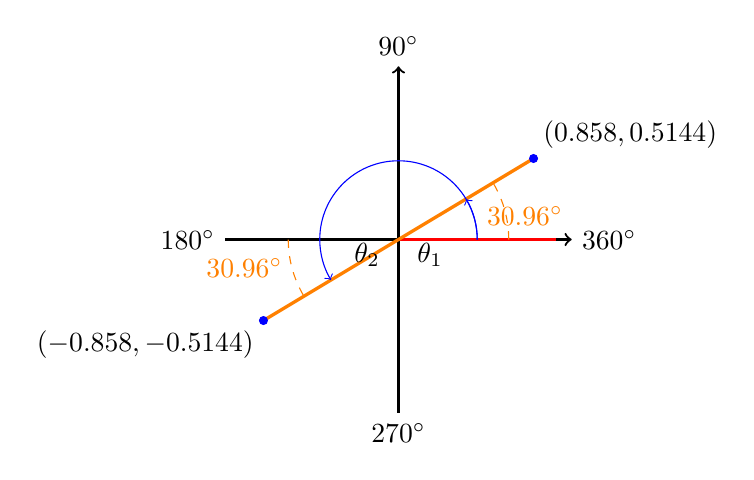
\begin{tikzpicture}[scale=2]
          % Axes
          \draw[thick,->] (-1.1,0) -- (1.1,0) node[right] {$360^\circ$};
          \draw[thick,->] (0,-1.1) -- (0,1.1) node[above] {$90^\circ$};
          \draw[thick] (-1,0) -- (-1.1,0) node[left] {$180^\circ$};
          \draw[thick] (0,-1) -- (0,-1.1) node[below] {$270^\circ$};
          % Initial arm
          \draw[very thick,red] (0,0) -- (1,0);
          % Terminal arm Q1
          \draw[very thick,orange] (0,0) -- ({cos(30.96)},{sin(30.96)});
          % Terminal arm Q3
          \draw[very thick,orange] (0,0) -- ({cos(210.96)},{sin(210.96)});
          % Reference angle arc Q1
          \draw[dashed,orange] (0.7,0) arc (0:30.96:0.7);
          % Reference angle arc Q3
          \draw[dashed,orange] ({0.7*cos(180)},{0.7*sin(180)}) arc (180:210.96:0.7);
          % Arrows for angle sweep
          \draw[->,blue] (0.5,0) arc (0:30.96:0.5);
          \draw[->,blue] (0.5,0) arc (0:210.96:0.5);
          % Points
          \filldraw[blue] ({cos(30.96)},{sin(30.96)}) circle (0.025);
          \filldraw[blue] ({cos(210.96)},{sin(210.96)}) circle (0.025);
          % Labels
          \node[above right] at ({cos(30.96)},{sin(30.96)}) {$(0.858,0.5144)$};
          \node[below left] at ({cos(210.96)},{sin(210.96)}) {$(-0.858,-0.5144)$};
          \node[orange,right] at (0.5,0.15) {$30.96^\circ$};
          \node[orange,left] at ({0.7*cos(195)},{0.7*sin(195)}) {$30.96^\circ$};
          \node at (0.2,-0.1) {$\theta_1$};
          \node at (-0.2,-0.1) {$\theta_2$};
        \end{tikzpicture}
        \end{center}
    \end{tcolorbox}
\end{frame}

% Practice: Find coordinates for given trig values
\begin{frame}{Practice: Find Coordinates}
    \begin{tcolorbox}[colback=lightgray,colframe=accent,title=Practice]
        \footnotesize
        Given the trig value, show the angle in standard position and the coordinates of $P$ on the unit circle:
        \begin{itemize}
            \item $\sin\theta = -2/5$
            \item $\sin\theta = -6/11$
            \item $\tan\theta = 3/5$
        \end{itemize}
    \end{tcolorbox}
\end{frame}

% Practice: Solve for $\theta$ (sinθ = -4/7)
\begin{frame}{Practice: Solve for $\theta$}
    \begin{tcolorbox}[colback=lightgray,colframe=accent,title=Practice]
        \footnotesize
        Solve for $\theta$ given $\sin\theta = -4/7$.
    \end{tcolorbox}
\end{frame}

\begin{frame}{Practice: Solve for $\theta$}
    \begin{tcolorbox}[colback=lightgray,colframe=accent,title=Solution]
        \footnotesize
        $\sin\theta = -4/7$ (negative)\\
        $\theta$ in Q3 and Q4\\
        $\theta_1 = 360^\circ - \sin^{-1}(4/7) \approx 209.46^\circ$\\
        $\theta_2 = 360^\circ + \sin^{-1}(4/7) \approx 330.54^\circ$
        
        \begin{center}
        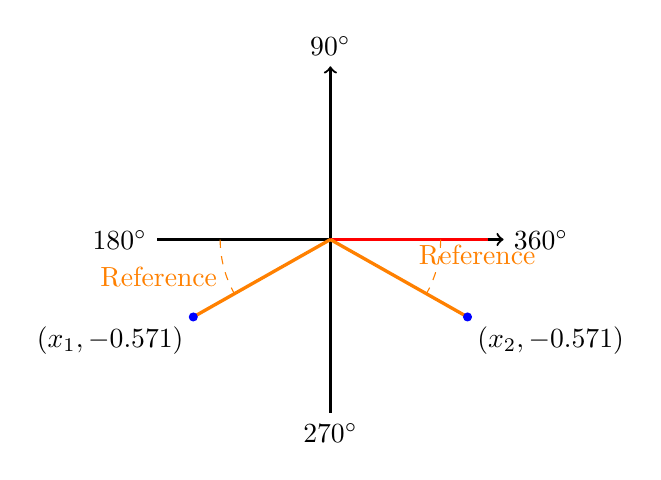
\begin{tikzpicture}[scale=2]
          % Axes
          \draw[thick,->] (-1.1,0) -- (1.1,0) node[right] {$360^\circ$};
          \draw[thick,->] (0,-1.1) -- (0,1.1) node[above] {$90^\circ$};
          \draw[thick] (-1,0) -- (-1.1,0) node[left] {$180^\circ$};
          \draw[thick] (0,-1) -- (0,-1.1) node[below] {$270^\circ$};
          % Initial arm
          \draw[very thick,red] (0,0) -- (1,0);
          % Terminal arm Q3
          \draw[very thick,orange] (0,0) -- ({cos(209.46)},{sin(209.46)});
          % Terminal arm Q4
          \draw[very thick,orange] (0,0) -- ({cos(330.54)},{sin(330.54)});
          % Reference angle arc Q3
          \draw[dashed,orange] ({0.7*cos(180)},{0.7*sin(180)}) arc (180:209.46:0.7);
          % Reference angle arc Q4
          \draw[dashed,orange] (0.7,0) arc (0:-29.46:0.7);
          % Points
          \filldraw[blue] ({cos(209.46)},{sin(209.46)}) circle (0.025);
          \filldraw[blue] ({cos(330.54)},{sin(330.54)}) circle (0.025);
          % Labels
          \node[below left] at ({cos(209.46)},{sin(209.46)}) {$(x_1, -0.571)$};
          \node[below right] at ({cos(330.54)},{sin(330.54)}) {$(x_2, -0.571)$};
          \node[orange,left] at ({0.7*cos(200)},{0.7*sin(200)}) {Reference};
          \node[orange,right] at (0.5,-0.1) {Reference};
        \end{tikzpicture}
        \end{center}
    \end{tcolorbox}
\end{frame}

% Practice: Solve for $\theta$ (cosθ = 5/13)
\begin{frame}{Practice: Solve for $\theta$}
    \begin{tcolorbox}[colback=lightgray,colframe=accent,title=Practice]
        \footnotesize
        Solve for $\theta$ given $\cos\theta = 5/13$.
    \end{tcolorbox}
\end{frame}

\begin{frame}{Practice: Solve for $\theta$}
    \begin{tcolorbox}[colback=lightgray,colframe=accent,title=Solution]
        \footnotesize
        $\cos\theta = 5/13$ (positive)\\
        $\theta$ in Q1 and Q4\\
        $\theta_1 = \cos^{-1}(5/13) \approx 67.38^\circ$\\
        $\theta_2 = 360^\circ - 67.38^\circ = 292.62^\circ$
        
        \begin{center}
        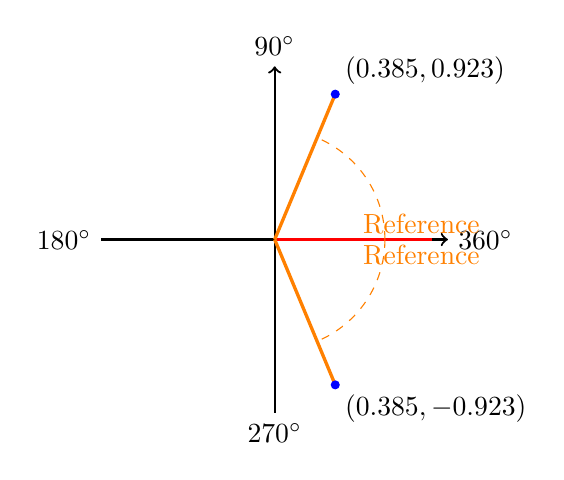
\begin{tikzpicture}[scale=2]
          % Axes
          \draw[thick,->] (-1.1,0) -- (1.1,0) node[right] {$360^\circ$};
          \draw[thick,->] (0,-1.1) -- (0,1.1) node[above] {$90^\circ$};
          \draw[thick] (-1,0) -- (-1.1,0) node[left] {$180^\circ$};
          \draw[thick] (0,-1) -- (0,-1.1) node[below] {$270^\circ$};
          % Initial arm
          \draw[very thick,red] (0,0) -- (1,0);
          % Terminal arm Q1
          \draw[very thick,orange] (0,0) -- ({cos(67.38)},{sin(67.38)});
          % Terminal arm Q4
          \draw[very thick,orange] (0,0) -- ({cos(292.62)},{sin(292.62)});
          % Reference angle arc Q1
          \draw[dashed,orange] (0.7,0) arc (0:67.38:0.7);
          % Reference angle arc Q4
          \draw[dashed,orange] (0.7,0) arc (0:-67.38:0.7);
          % Points
          \filldraw[blue] ({cos(67.38)},{sin(67.38)}) circle (0.025);
          \filldraw[blue] ({cos(292.62)},{sin(292.62)}) circle (0.025);
          % Labels
          \node[above right] at ({cos(67.38)},{sin(67.38)}) {$(0.385,0.923)$};
          \node[below right] at ({cos(292.62)},{sin(292.62)}) {$(0.385,-0.923)$};
          \node[orange,right] at (0.5,0.1) {Reference};
          \node[orange,right] at (0.5,-0.1) {Reference};
        \end{tikzpicture}
        \end{center}
    \end{tcolorbox}
\end{frame}

\end{document} 